\section{Unterschiedliche Arten der Applikation für mobile Engeräte}
Für die Programmierung von Multi-Plattform-Applikationen gibt es verschiedene Klassen, in die die Entwicklungsmethoden eingeordnet werden können. Dabei unterscheiden verschiedene Autoren unterschiedliche Klassen. In dieser Arbeit wird daher der von Delia et al \cite{IEEE_development_classes} definierten Einteilung gefolgt, da ihre Definition einen vernünftiger Pfad zwischen zu detailliert und zu allgemein darstellt. Im Folgenden sollen diese vorgestellt und auf einige Aspekte der einzelnen Klassen eingegangen werden.

\subsection{Native Applikationen}
Native Applikationen werden entwickelt, um auf einer bestimmten Plattform installiert zu werden. Der Quellcode wird dafür zu ausführbaren Code übersetzt, der spezifisch für die gewählte Plattform ist \cite{IEEE_development_classes}.
Die Programmierung wird in der für die Plattform typischen Programmiersprache geschrieben und ist dadurch nur für eine Plattform nutzbar. Es gibt folglich für jede Plattform einen eigenen Quellcode. Um etwa eine native Android App zu entwickeln, wird diese in Kotlin programmiert und im Anschluss in Kotlin-Bytecode übersetzt. Dieser Bytecode ist dabei nur auf Android Geräten ausführbar.

Der Vorteil der nativen Entwicklung ist, dass die Funktionen der verschiedenen Plattform optimal genutzt werden können, da die definierten eindeutig definierten Schnittstellen lediglich aufgerufen werden müssen. So ist etwa eine Nutzung der Kamera, GPS, Beschleunigungssensoren, Kalender und anderen, einfach und effizient. Dabei ist die Ausführung nicht nur schnell, sondern kann auch in einem Hintergrundprozess gestartet werden \cite{IEEE_development_classes}. Dazu kommt, dass das Aussehen der Applikation und die Benutzerschnittstellen ähnlich zu der unterstützten Plattform ist, da die selben Elemente genutzt werden. So entsteht für den Nutzer ein geschlossenes System, das leichter zu bedienen ist, da es kaum Unterschiede in Struktur, Design, Aufbau oder auch Benutzung gibt \cite{IEEE_Khackouch_Al}.

Ein Nachteil der nativen Entwicklung ist der Aufwand und die damit verbundenen Kosten, um für die verschiedenen Plattformen eine Applikation anbieten zu können. Denn sie muss für jede Plattform einzeln entwickelt werden. So können die Kosten für eine Plattform mit der Anzahl der abzudeckenden Plattformen multipliziert werden, um die Gesamtkosten zu erhalten \cite{IEEE_Khackouch_Al}. Doch nicht nur die Programmierung ist ein Kostenfaktor. So nennen Delia et al auch das Testen, Abändern und Verteilen neuer Version als Faktoren, die auf jeder einzelnen unterstützten Plattform auftreten \cite{IEEE_development_classes}. Um die Kosten zu verringern, werden deswegen anfänglich nur einzelne Plattformen ausgewählt, wodurch jedoch die Reichweite der Anwendung sinkt.

\subsection{Web-Applikationen}
Web-Applikationen sind Applikationen, die im Netz verfügbar sind. Sie sind darauf ausgelegt, als Webseiten auf einem Server zu laufen und dann über den Browser der Geräte aufgerufen zu werden. Dieser Ansatz ist einfach für den Nutzer, da eine Webseite sofort für jeden Nutzer verfügbar ist, sobald sie auf dem Server gestartet wurde. Daher muss sie nicht erst auf dem Gerät installiert werden um sie zu nutzen \cite{IEEE_Khackouch_Al}. Sie muss auch nur einmal entwickelt werden, da sie auf allen Geräten mit einem Browser und einer Internetverbindung aufgerufen werden kann. So können alle Plattformen mit nur einer Entwicklung abgedeckt werden \cite{IEEE_development_classes}.

Wie bereits erwähnt, wird ein Code für alle Plattformen geschrieben. Dies ist von Vorteil, wenn die Entwicklungskosten stark eingeschränkt sind. Ein weiterer Vorteil ist, dass Updates dem Nutzer direkt nach einem Neustart des Servers zur Verfügung stehen, da es nicht erst an die Geräte verteilt und dann installiert werden muss \cite{IEEE_Khackouch_Al}. Des weiteren können mittlerweile selbst Personen ohne Programmiererfahrung Webseiten erstellen, da durch Firmen wie Squarespace\footnote{https://de.squarespace.com/} die Erstellung, auf die Auswahl einer Vorlage und einigen Anpassungen am Design, beschränkt ist. 
Außerdem kann der Code wiederverwendet um etwa eine hybride Applikation zu erstellen \cite{IEEE_Khackouch_Al}.  

Jedoch ist die nutzbare Funktionalität der Plattform, durch die Nutzung des Browsers stark eingeschränkt. Dabei kann lediglich die Funktionalität genutzt werden, auf die der Browser zugriff hat \cite{Phyo}. Dazu kommt, dass bei einer fehlenden Internetverbindung die Anwendung nicht genutzt werden kann und bei einer langsamen Internetverbindung die Performance durch erhöhte Ladezeiten sinkt \cite{IEEE_Khackouch_Al}. Außerdem müssen Webanwendungen zur Nutzung auf Smartphones angepasst werden. So sind Smartphones etwa höher als breit und haben daher weniger Platz in der Menüleiste als etwa bei einer Nutzung an einem Computer. Daher müssen Webanwendungen auf unterschiedliche Seitenverhältnisse und Auflösungen reagieren können und ein angepasstes Designs für die Plattformen zur Verfügung stellen \cite{Serrano_mobile}.

Web-Applikationen sind in den letzten Jahren, durch die Verfügbarkeit von schnellen Internetverbindungen in fast allen Teilen der Welt, einfacher nutzbar geworden.
Im Schnitt stieg die mobile Bandbreite zwischen 2017 und 2021 um 59,5\% beziehungsweise von knapp 20 Mbps auf 55 Mbps \footnote{https://www.ookla.com/articles/global-index-2019-internet-report}.
Jedoch ergab eine Studie von Yoram Wurmser \cite{report_webusage}, dass während der Nutzung des Smartphones, amerikanische Erwachsene etwa 89\% der Zeit in Applikationen und gerade einmal 11\% in einem Browser verbringen.

\subsection{Hybride Applikationen}
Eine Klasse die viel mit der vorherigen Klasse zu tun hat, sind die hybriden Applikationen.
Sie nutzen Web-Technologien, also HTML, Javascript und CSS, werden jedoch in einem Container und nicht im Browser des Geräts ausgeführt.
Dieser hat dabei über eine Schnittstelle Zugriff auf die Funktionalität der Plattform \cite{IEEE_development_classes}.

\begin{figure}[ht]
  \centering
  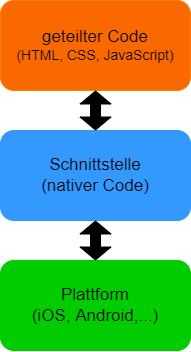
\includegraphics[height=7cm,keepaspectratio]{images/hybrid_architecture.drawio.png} 
  \caption{Architektur einer hybriden Applikationen}
  \label{fig:hybrid_architecture}
\end{figure}

Wie in Abbildung \ref{fig:hybrid_architecture} zu sehen ist, besteht diese Art von Applikation aus zwei Teilen.
Der erste Teil ist ein geteilter Code, der mit Web-Technologien erstellt wird und sowohl die UI und Applikationslogik enthält. Dieser Code kann dabei sowohl lokal als auch auf einem Server gespeichert sein \cite{2017hybrid_approach_end}.
Der zweite Teil ist eine Schnittstelle, die in nativen plattformspezifischen Code geschrieben ist. Sie kann komplett selbst geschrieben werden oder durch Technologien wie Cordova\footnote{https://cordova.apache.org/} definiert und für die unterstützten Plattformen kompiliert werden. Die Schnittstelle bietet dabei eine beidseitige Kommunikation zwischen der Plattform und ihrer dazugehörigen Funktionalitäten und der Applikation \cite{ELKASSAS2017163}. Außerdem ist sie dafür verantwortlich, die Applikation auf dem Gerät anzuzeigen. 

Grundsätzlich hat diese Klasse die gleichen Vor- und Nachteile wie Web-Applikationen, da sie zu einem großen Teil aus der selben Technologie besteht, die in einer eigenen App angezeigt wird. Jedoch kann sie mit der richtigen Implementierung, eine offline Funktionalität erreichen. Dazu kommt, dass die Applikation durch die Schnittstelle die native Funktionalität nutzen und auf einem Gerät installiert werden kann. Außerdem kann der Code sowohl auf den verschiedenen Plattformen, als auch in anderen Technologien wiederverwendet werden \cite{IEEE_development_classes}. Jedoch entsteht durch den zusätzlichen Web-Container, der geladen werden muss um die UI anzuzeigen, eine erhöhte Ladezeit, die sich negativ auf die Performance der Applikation auswirkt \cite{IEEE_development_classes}. Außerdem entsteht durch die Nutzung von Javascript eine mögliche Schwachstelle der Applikationen \cite{javascript_dangerous}. 

\subsection{Interpretierte Cross-Plattform Applikationen}
Bei interpretieren Cross-Plattform Anwendungen schreibt der Entwickler einen Code, der dann mithilfe eines Interpreters während der Laufzeit in ausführbaren Code übersetzt wird. Das bedeutet, dass die auf dem Gerät installierte Anwendung aus zwei Teilen besteht. Einerseits einem nativen Teil, oftmals Frameworkcode, der zum Übersetzen der eigentlichen Anwendung benötigt wird. Andererseite einen Cross-Plattform Teil, der aus der Anwendungslogik besteht \cite{IEEE_development_classes}.

Der Unterschied zu den hybriden Applikationen besteht dabei darin, dass etwa die Benutzeroberfläche nicht so angezeigt wird, wie sie im Code definiert ist, sondern während der Laufzeit in eine nativ \ac{UI} übersetzt wird, bevor sie angezeigt wird. Dadurch wird eine Nutzung von nativen Elementen möglich, obwohl die Anwendung eigentlich in einer anderen Sprache definiert ist \cite{IEEE_development_classes}. Dazu kommt, dass interpretierte Anwendungen auf allen Plattformen ausgeführt werden kann, die von dem entsprechenden Interpreter unterstützt werden \cite{server_side}.

Genau das kann jedoch auch zum Problem werden, wenn die gewünschte Plattform nicht unterstützt wird. Außerdem ist durch die Interpretierung während der Laufzeit dieser Ansatz langsamer als andere, da jede Zeile vor Ausführung erst durch den Interpreter übersetzt werden muss und somit eine extra Latenz zwischen jedem einzelnen Aufruf und dessen Ausführung entsteht \cite{server_side}.

\subsection{Cross-kompilierte Applikationen}
Das Problem der zusätzlichen Latenz kann dafür in der Klasse der Cross-kompilierten Anwendungen verhindert werden. Bei diesem Ansatz wird zwar während der Entwicklung ebenfalls nur ein Quellcode geschrieben, jedoch wird dieser bereits vor Veröffentlichung in nativen Code übersetzt. Dadurch muss der übersetzungsprozess nur einmal durchgeführt werden und nicht wie bei dem interpretierten Ansatz bei jedem Aufruf. Um dies zu erreichen, wird ein Cross-Compiler benötigt, der für mehrere unterschiedliche Plattformen Kompilate erzeugt \cite{mobiledraft_cross_plattform}. Somit kann aus einem Code eine Anwendung für jede Plattform gebaut werden, die nur aus nativem Code besteht, und sich somit für das Betriebssystem nicht von einer nativen Anwendung unterscheidet \cite{IEEE_development_classes}.Im Vergleich zur interpretieren Anwendung kann außerdem die App-Größe reduziert werden, da kein zusätzlicher Übersetzer benötigt wird \cite{mobiledraft_cross_plattform}.

Auch bei diesem Ansatz ist die Funktionalität und die Zahl der unterstützten Plattformen von der genutzten Technologie abhängig. Viele dieser Ansätze nutzen außerdem eine eigene Programmiersprache, sodass eine Wiederverwendung des Codes für einen anderen Ansatz erschwert wird. So wird bei den cross-kompilier Frameworks Flutter\footnote{https://flutter.dev/} die Sprache Dart\footnote{https://dart.dev/} und bei Xamarin\footnote{https://dotnet.microsoft.com/en-us/apps/xamarin} Lua\footnote{https://www.lua.org/} genutzt.


\subsection{Gemischter Ansatz}
Im Gegensatz zu Delia et al, soll in dieser Arbeit die Applikationsklassen um einen weiteren Ansatz erweitert werden, wie ihn auch Khachouch et al \cite{IEEE_Khackouch_Al} in ihrere Arbeit aufführen. Sie definieren einen gemischten Ansatz, da die verschiedenen Ansätze auch kombiniert werden können, um die Vorteile verschiedener Klassen zu kombinieren. So wird in dieser Arbeit etwa ein gemischter Ansatz aus einer hybriden und einer Cross-kompilierten Applikation.
